\documentclass[12pt, fullpage,letterpaper]{article}

\usepackage[margin=1in]{geometry}
\usepackage{url}
\usepackage{amsmath,amsthm,amssymb}
\usepackage{undertilde}
\usepackage{cancel}
\usepackage{pgfplots}
\usepackage{algorithm, algorithmic}
\usepackage{xcolor}
\usepgfplotslibrary{polar}
\usepgflibrary{shapes.geometric}
\usetikzlibrary{calc}

\pgfplotsset{my style/.append style={axis x line=middle, axis y line=
middle, xlabel={$x$}, ylabel={$y$}, axis equal }}

\newcommand{\semester}{Fall 2015}
\newcommand{\assignmentId}{5}
\newcommand{\releaseDate}{Nov 20, 2015}
\newcommand{\dueDate}{Dec 8, 2015}

\newcommand{\bx}{{\bf x}}
\newcommand{\bw}{{\bf w}}
\newcommand{\Grad}[1]{\vec{\nabla} #1 }
\renewcommand{\P}[1]{\left( #1\right)}
\title{CS 5350/6350: Machine Learining \semester}
\author{Homework \assignmentId\\Christopher Mertin}
\date{Handed out: \releaseDate\\
  Due date: \dueDate}

\begin{document}
\maketitle
{\large\bf Notation}

It is important that I define two different notations that are used in this homework assignment. I used this notation to make the math work easier, though my final results I remove this notation

{\bf Einstein Summation Notation}

This simply removes the sum as the sum is \underline{understood} for the context of the problem. Example:

\[
\sum_{i=1}^{n} \zeta_{i} = \zeta_{i}
\]

{\bf Mertin Product Notation}

This removes the product symbol infront of some terms as it is \underline{understood} from the context of the problem. I made a variation to make it different when compared to {\em Einstein Summation Notation} so you can tell the difference (note the tilde)

\[
\prod_{i=1}^{n}\zeta_{i} = \utilde{\zeta_{i}}
\]

\textcolor{red}{{\bf Side Note:} I talked with Dr. Srikumar and he mentioned that for this assignment it was alright if I went over by a few pages and points wouldn't be taken off. I condensed my answers as much as I could.}

{\large \bf Na\"{i}ve-Bayes}

\begin{enumerate}
\item The weight vector can be defined as such $\mathbf{w}=\left(1,1,1,1,1,1,1\right)^{T}$, with the bias, $\theta$, can be defined such that $\theta = -3$. This will give the result that if $\mathbf{w}^{T}\mathbf{x}_{i}+\theta\geq 0$, then $y=1$, otherwise $y=-1$. This will result in the bounds such that if at least $3$ of the components are $1$, then the result would be $y=1$.
\item Let $x_{i}$ be the $i^{th}$ input of the data in the cube for $i = \{1,2,\ldots,n\}$. We can find the most probable hypothesis by
\begin{align}
p(h|\mathcal{D}) &= \text{arg}\max_{h\in H}p\left(y_{i}|x_{i}\right)\\
\intertext{The question states that we are sampling from a normal distribution over the cube, we can represent all the data in the following way}
 &\Rightarrow \text{arg}\max_{y\in \{0,1\}}p(y)\prod_{i=1}^{7}p\left(x_{i}|y\right)\\
\intertext{which expands into the form}
\max &\left[ p(0)\prod_{i=1}^{7}p\left(x_{i}|0 \right), p(1)\prod_{i=1}^{7}p\left(x_{i}|1 \right)\right]\\
p(0) &= \text{probability that at least 5 elements are 0}\\
&= \left(\frac{1}{2}\right)^{7}\sum_{i=5}^{7}{7 \choose i} = \frac{29}{128}\\
p(1) &= 1 - p(0) = \frac{99}{128}
\intertext{We now need to define $p(x_{i}=0|y)$ and $p(x_{i}=1|y)$, for $y = \{ 0, 1\}$. These would be the same for all values of $i$ since they come from the same distribution}
p(x_{i}|0) &= \frac{p(x_{i})p(0|x_{i})}{p(0)}\label{eq:all}\\
\intertext{For $x_{i}=1$, we need to calculate the probability of $p(0|x_{i}=1)$, which is the probability of {\em at least} 5 of the remaining 6 $x_{i}$'s being 0}
p(0|x_{i}=1) &= \left( \frac{1}{2}\right)^{6}\left[ {6 \choose 5} + {6 \choose 6}\right] = \frac{7}{64}\\
\intertext{Now we can calculate $p(x_{i}=1|0)$ from Equation (\ref{eq:all})}
p(x_{i}=1|0) &= \frac{\frac{1}{2}\frac{7}{64}}{\frac{29}{128}} = \frac{7}{29}
\intertext{Where we can do the same thing for $x_{i}=0$, which would be the probability of at least 4 of the remaining 6 being 0}
p(0|x_{i}=0) &= \left(\frac{1}{2}\right)^{6}\left[ \sum_{i=4}^{6}{6 \choose i}\right] = \frac{22}{64}
\intertext{where from here we can calculate $p(x_{i}=0|0)$ from Equation (\ref{eq:all}) again as being}
p(x_{i}=0|0) &= \frac{\frac{1}{2}\frac{22}{64}}{\frac{29}{128}} = \frac{22}{29}
\intertext{Finally, we need to calculate it for $y=1$, whcih can be done as follows}
p(1|x_{i}=1) &= 1 - p(0|x_{i}=1) = 1-\frac{7}{64} = \frac{57}{64}\\
p(1|x_{i}=0) &= 1 - p(0|x_{i}=0) = 1-\frac{22}{64} = \frac{42}{64}\\
\intertext{Leading to the final results of}
p(x_{i}=1|1) &= \frac{\frac{1}{2}\frac{57}{64}}{\frac{99}{128}} = \frac{57}{99}\\
p(x_{i}=0|1) &= \frac{\frac{1}{2}\frac{42}{64}}{\frac{99}{128}} = \frac{42}{99}\\
\intertext{From these we can build the hypothesis}
h(\mathbf{x}) &= \text{arg}\max_{y\in \{0,1\}} \frac{29 + 70y}{128}\prod_{i=1}^{7}\frac{42 + 15\mathbf{x}_{i}}{99}y - \frac{22 - 15\mathbf{x}_{i}}{29}(y-1)\label{eq:hyp}
\end{align}
\item This can be proven via {\em proof by contradiction}. Assume we have the vector $\mathbf{x}=(0,0,0,1,0,0,1)^{T}$ and that the hypothesis in the answer to the previous question correctly classifies the data. From the first question, we know that this should be classified as $y=0$. We can test this to verify
\begin{align}
h(\mathbf{x}) &= \max_{y\in \{0,1\}}\left\{ \begin{array}{l l r}
\frac{29}{128}\left[ \left(\frac{22}{29}\right)^{5}\left(\frac{7}{29}\right)^{2} \right]\approx & 0.003317 & (y=0)\\
\frac{99}{128}\left[ \left(\frac{57}{99}\right)^{2}\left(\frac{42}{99}\right)^{5} \right]\approx & 0.003524 & (y=1)
\end{array}\right.
\end{align}
which the hypothesis would choose the largest number which would be $y=1$, which isn't true as it should be $y=0$. This is a contradiction, therefore it doesn't describe this function.
\item No, the na\"{i}ve bayes assumptions are not satisfied by $f_{TH(3,7)}$. The assumption that is made is that $\mathbf{x}_{i}$ is independent for each value of $i$, which isn't actually the case. Any of the probability calculations should include the probability of the other features as well.
\end{enumerate}

{\large \bf EM}

\begin{enumerate}
\item The joint probability density function of $p(x_{i}|\lambda)$ is the product of each probabilty for $i = \{1,2,\ldots,n\}$
\begin{align}
p(x|\lambda) &= \prod_{i=1}^{n}p(x_{i}|\lambda) = \prod_{i=1}^{n}\frac{\lambda^{x_{i}}e^{-\lambda}}{x_{i}!}\\
&= \frac{\lambda^{\sum_{i=1}^{n}x_{i}}e^{-n\lambda}}{\prod_{i=1}^{n}x_{i}!}
\intertext{which we can take the log of now to get the log-likelihood function}
\ell(\theta) &= \log\left[ \frac{\lambda^{\sum_{i=1}^{n}x_{i}}e^{-n\lambda}}{\prod_{i=1}^{n}x_{i}!}\right]\\
&= \log\left[ \left(\sum_{i=1}^{n}x_{i}\right)\log(\lambda) + (-n\lambda)\log(e) - \prod_{i=1}^{n}\log(x_{i}!) \right]\\
\intertext{where we want to maximize $\lambda$, so we take $\frac{\partial \ell(\theta)}{\partial \lambda}$ and set it equal to zero}
0 &= \frac{\partial \ell(\theta)}{\partial \lambda} = \frac{\sum_{i=1}^{n}x_{i}}{\lambda} - n\\
n\lambda &= \sum_{i=1}^{n}x_{i}\\
\lambda &= \frac{1}{n}\sum_{i=1}^{n}x_{i}
\end{align}

\item The data that is given to us is such that $i=\{1,2,\ldots,n\}$ and $j=\{1,2,\ldots,m\}$, where $m$ is the number of records and $n$ is the number of lanes. The generative model that can be used for this is

\begin{align}
h(\mathbf{x}) &= \text{arg}\max_{y\in \{S,T\}}p(y)\prod_{j=1}^{m}\sum_{i=1}^{n}p(y|x_{i})\\
&= \text{arg}\max_{y\in \{S,T\}}p(y)\prod_{j=1}^{m}\sum_{i=1}^{n}\frac{p(x_{i}|y)}{p(x_{i})}\label{eq:whocares}
\intertext{We don't know the distribution of the $m$ records, but we do know that there is a probability $\eta$ that a record represents data from Smith's and $(1-\eta)$ that it represents data from Trader Joe's. We can calculate the maximum likelyhood by Equation~(\ref{eq:whocares}) by splitting the $\max$ for $y\in\{S,T\}$. The base equation used to represent the probability of {\em each record} is}
h(\mathbf{x}) &= \text{arg}\max_{y\in\{S,T\}}\sum_{i=1}^{n}p(y)p(x_{i}|y)
\intertext{which would be for a single data set. Therefore, to account for each record, the resulting equation would be}
h(\mathbf{x}) &= \text{arg}\max_{y\in\{S,T\}}\left\{\begin{array}{l l}\eta\prod_{j=i}^{m}\frac{\lambda_{S}^{\sum_{i=1}^{n}x_{j,i}}e^{-n\lambda_{S}}}{\prod_{i=1}^{n}x_{j,i}!}\\
(1-\eta)\prod_{j=i}^{m}\frac{\lambda_{T}^{\sum_{i=1}^{n}x_{j,i}}e^{-n\lambda_{T}}}{\prod_{i=1}^{n}x_{j,i}!} \end{array} \right.
%\intertext{where each result would be calculated for each record and the largest would be chosen. On the one that is the largest, $\lambda_{S}$ and $\lambda_{T}$ would be updated in the following way}
%\lambda_{\xi\in\{S,T\}} &= \frac{1}{k\cdot n}\sum_{j=1}^{k}\sum_{i=i}^{n}x_{j,i}\\
%\intertext{where $k$ is the total number of current records for which $\lambda_{\xi}$ was the maximum and belonging to either $S$ or $T$ (whichever was maximum and needs to be updated). Following this, the parameters that are needed are $\eta$ and an initial value for $\lambda_{\xi}$ to start the process which will update $\lambda_{S}$ and $\lambda_{T}$.}\nonumber
\end{align}
To use $h(\mathbf{x})$ to classify the data, the parameters we would need would be $\eta$ to tell the probability of which belongs to $S$ or $T$, and we would need an initial value of $\lambda$ which would be the value that we use in the first iteration for {\em both} $\lambda_{S}$ and $\lambda_{T}$. One way to do this would be to either pick a random number or to take the average of the first record. The way that the EM algorithm can be used to cluster the records is described in the next part.


\item In order to cluster the data into two sets, we would take the first record and plug it into the two different cases of $h(\mathbf{x})$ and the largest result would correspond to that label. 

For example, if the $k^{th}$ record when plugged into $h(\mathbf{x})$ is largest for $y=S$, then that data set would be treated as belonging to Smith's. Following this, we would then need to update $\lambda_{S}$ in the following way

\begin{align}
\lambda_{S} &= \frac{1}{k\cdot n}\sum_{j=1}^{k}\sum_{i=1}^{n}x_{j,i}
\end{align}

where $k$ represents the number of records that corresponded to $S$. We would iterate through all $m$ records to get this result and continually update $\lambda_{S}$ and $\lambda_{T}$ until we got the best fit of the distributions.

\item We can find the decision boundary in the following way. The boundary line is defined as:
\begin{align}
p(\xi ) &= \frac{p(y=S|x_{j,i})}{p(y=T|x_{j,i})} = \frac{p(x_{j,i}|y=S)p(T)}{p(x_{j,i}|y=T)P(S)} > 1\\
\intertext{where $p(\xi)$ is being used to shorten the notation. We can plug in what we know for $p\left(x_{j,i}|y=\{S,T\}\right)$, $p(S)$, and $p(T)$, resulting in}
p(\xi) &= \frac{(1-\eta)}{\eta}\frac{\frac{    \lambda_{S}^{\sum_{i=1}^{n}x_{j,i}}e^{-n\lambda_{S}}}{\prod_{i=1}^{n}x_{j,i}!}    }{ \frac{\lambda_{T}^{\sum_{i=1}^{n}x_{j,i}}e^{-n\lambda_{T}}}{\prod_{i=1}^{n}x_{j,i}!}}\\
\intertext{Which can be simplified in the following way. Since the exponential terms are independent of $j$, they can be pulled outside of the project. And since the denominators are the same in each of the probabilities, we can cancel them. The following is the much more simplified result using {\em Einstein Summation Notation} and {\em Mertin Product Notation}}
p(\xi) &= \underbrace{\frac{(1-\eta)}{\eta}}_{\alpha}\underbrace{\frac{e^{-nm\lambda_{S}}}{e^{-nm\lambda_{T}}}}_{\beta}\underbrace{\utilde{\frac{\lambda_{S}^{x_{j,i}}}{\lambda_{T}^{x_{j,i}}}}}_{\gamma_{j,i}}>1\\
\intertext{which the substitutions in the underbraces can be made to make the simplification process easier, resulting in}
p(\xi) &= \alpha\beta\utilde{\gamma_{j,i}}>1\\
\intertext{Following this, the $\log$ of both sides can be taken, resulting in}
p(\xi) &= \log(\alpha) + \log(\beta) + \log\left(\utilde{\gamma_{j,i}}\right) > \log(1)\\
p(\xi) &= \log(\alpha) + \log(\beta) + \log\left(\utilde{\gamma_{j,i}}\right) > 0\\
\intertext{Where we can plug in back the values of $\alpha$, $\beta$, and $\gamma_{j,i}$}
p(\xi) &= \log\left(\utilde{\lambda_{S}^{x_{j,i}}}\right) - \log\left(\utilde{\lambda_{T}^{x_{j,i}}}\right) + \log\left(\frac{(1-\eta)}{\eta}\right) + \log\left(\frac{e^{-nm\lambda_{S}}}{e^{-nm\lambda_{T}}}\right)>0\\
p(\xi) &= \utilde{x_{j,i}\log\left(\frac{\lambda_{S}}{\lambda_{T}}\right)} + \log\left(\frac{(1-\eta)}{\eta}\right) + nm\left(\lambda_{T}-\lambda_{S}\right)>0\\
\intertext{where going back to the normal notation gives us the definition of the update}
p(\xi) &= \underbrace{\prod_{j=1}^{m}\sum_{i=1}^{n}x_{j,i}\log\left(\frac{\lambda_{S}}{\lambda_{T}}\right)}_{\mathbf{w}^{T}\mathbf{x}} + \underbrace{\log\left(\frac{(1-\eta)}{\eta}\right) + nm\left(\lambda_{T}-\lambda_{S}\right)}_{b}>0
\end{align}
\end{enumerate}

{\large \bf Experiment}

\begin{enumerate}
\item We can simply treat $\mathbf{w}$ as a variable and it becomes a normal differentiation problem
\begin{align}
f(\mathbf{x}_{i}) &= \log\P{1+\exp(-y_{i}\mathbf{w}^{T}\mathbf{x}_{i})}\\
\intertext{where we can perform a $u$-substition such as}
u &= 1 + \exp\left(-y_{i}\mathbf{w}^{T}\mathbf{x}_{i}\right)\\
\frac{\text{d}u}{\text{d}\mathbf{w}^{T}} &= -y_{i}\mathbf{x}_{i}\exp\left(-y_{i}\mathbf{w}^{T}\mathbf{x}_{i}\right)\\
\intertext{such that we can use these to differentiate $f(\mathbf{x}_{i})$ to be}
\frac{\partial f(\mathbf{x}_{i})}{\partial \mathbf{w}^{T}} &= \frac{\partial f(u)}{\partial \mathbf{w}^{T}}\frac{\partial u}{\partial \mathbf{w}^{T}} = \frac{-y_{i}\mathbf{x}_{i}}{\exp\left(y_{i}\mathbf{w}^{T}\mathbf{x}_{i}\right)+1}\label{eq:expo}
\intertext{To overcome instances of {\em overflow errors} in the computations, this equation can be rewritten in the following (equivalent) format from when Equation~(\ref{eq:expo}) overflows}
\frac{\partial f(\mathbf{x}_{i})}{\partial \mathbf{w}^{T}} &= \frac{(-y_{i}\mathbf{x}_{i})\cdot \exp(-y_{i}\mathbf{w}^{T}\mathbf{x}_{i})}{1 + \exp(-y_{i}\mathbf{w}^{T}\mathbf{x}_{i})}
\end{align}

\item We want the weight vector that minimizes our function, $J(\mathbf{w})$, so we need to take the gradient of it, but first we can {\em simplify} $J(\mathbf{w})$ to make the computation easier, which results in

\begin{align}
J(\mathbf{w}) &= \sum_{i=1}^{n}\log\P{1+\exp(-y_{i}\mathbf{w}^{T}x_{i})}+\frac{\mathbf{w}^{T}\mathbf{w}}{\sigma^{2}}\\
&= \sum_{i=1}^{n}\log\P{1+\exp(-y_{i}\mathbf{w}^{T}x_{i})}+\frac{\left|\left|\mathbf{w}\right|\right|^{2}}{\sigma^{2}}\\
\intertext{where we can take the derivative of this with respect to $\mathbf{w}$ and drop the summation since we're treating each record as the {\em only} data point. The first term is the same as the result in Equation~(\ref{eq:expo}) so only the second term needs to be differentiated with respect to $\mathbf{w}$}
\frac{\partial J(\mathbf{w})}{\partial \mathbf{w}}&= \frac{-y_{1}\mathbf{x}_{1}}{\exp(y_{1}\mathbf{w}^{T}\mathbf{x}_{1})+1} + 2\frac{\left|\left|\mathbf{w}\right|\right|}{\sigma^{2}}\label{eq:grad-J}
\end{align}

\item The pseudo code is represented in Algorithm~\ref{alg:SGD}, where $\gamma$ is the learning rate and there's a vector $\mathbf{x}_{i}\in\mathbb{R}^{n\times 1}$ in a set $S$ with $m$ different ``records.''
\begin{algorithm} % enter the algorithm environment
\begin{algorithmic}% enter the algorithmic environment
\STATE Initialize $\mathbf{w}_{(0)}\in\mathbb{R}^{n\times 1}$
\STATE Initialize list $\mathbf{w}_{list}\in\mathbb{R}^{T\times n}$
\FOR{$epoch=1,2,\ldots\ $\TO $T$}
\FORALL{$(\mathbf{x}_{i},y_{i})\in S$}
\STATE{Pick random example $(\mathbf{x}_{i},y_{i})$}
%\STATE{$J\left(\mathbf{w}_{(t)}\right) = \frac{1}{2}\mathbf{w}_{(t)}^{T}\mathbf{w}_{(t)}+C\sum_{i=1}^{n}\max\left[ 0, 1-y_{i}\mathbf{w}_{(t)}^{T}\mathbf{x}_{i,t} \right]$}
\STATE{Treat $(\mathbf{x}_{i},y_{i})$ as a full dataset and compute $\Grad{_{\mathbf{w}}J\left(\mathbf{w}_{(t)}\right)}$ from Equation~(\ref{eq:grad-J})}
\STATE{$\gamma_{(t)} = \frac{\gamma_{0}}{1+(\gamma_{0}\cdot t)/C}$}
\STATE{$\mathbf{w}_{(t+1)} = \mathbf{w}_{(t)} - \gamma_{(t)}\Grad{_{\mathbf{w}}J\left(\mathbf{w}_{(t)}\right)}$}
\ENDFOR
\STATE Append $\mathbf{w}$ from current $epoch$ to $\mathbf{w}_{list}$
\ENDFOR
\RETURN{$\min_{\mathbf{w}\in\mathbf{w}_{list}}\left\{ \sum_{i=1}^m \log\P{1+ \exp(-y_i\bw^T\bx_i)} + \frac{\left|\left|\mathbf{w}\right|\right|^{2}}{\sigma^2}  \right\}$}
\end{algorithmic}
\caption{Stochastic Gradient Descent$(S=\{(\mathbf{x}_{i},y_{i})\}_{m})$}
\label{alg:SGD}
\end{algorithm}

\item In order to implement Stochastic Gradient Descent, Algorithm~\ref{alg:SGD} was used. In doing so, there was a hyper parameter $\sigma$ which needed to be chosen. However, the ``learning rate'' $\gamma_{(t)}$ was dependent upon an initial value, $\gamma_{0}$, and $C=\sigma^{2}$. This learning rate changed over time and was defined as $\frac{\gamma_{0}}{1+(\gamma_{0}\cdot t)/(C)}$ which was important as the learning rate would decrease over time as the function presumably approached the maxima. These hyper parameters were {\em also} used to get the general range of what they should be. Table~\ref{table:hp_range} indicates the ranges that were initially trained over to see what the best values to use were. In the table, it only lists the minimum and maximum values, though the intermediary values were powers of 10 between the min and max. 

\begin{table}[!h]
\centering
\begin{tabular}{c | c c}
\hline\hline
{\bf Parameter} & {\bf Min} & {\bf Max}\\
\hline
$\sigma$ & $10^{-10}$ & $10^{10}$\\
$\gamma_{0}$ & $10^{-10}$ & $10^{10}$\\
\hline
\end{tabular}
\caption{Hyper-parameter Cross Validation Ranges}
\label{table:hp_range}
\end{table}

Using these ranges, 10-fold cross validation was implemented where the number of epochs for the cross validation was 10. This got the best values for each of the data sets which can be seen in Table~\ref{table:acc_orig} and Table~\ref{table:acc_scaled}, which show the top 5 parameters for each set. For some reason that is not known, the values of $\sigma$ and $\gamma_{0}$ were incredibly large for the best results, which are reflected in the corresponding tables. From here, the values that had the best accuracy were chosen for each file and run over the whole training set. The data set from this large cross validation was included in the archive file labeled \verb~longrun_output.dat~ so that you can see these results without running it over the large sets as it took more than 3 hours to run.

\begin{table}[!h]
\centering
\begin{tabular}{c c c}
\hline\hline
{\bf Accuracy} & $\boldsymbol{\gamma_{0}}$ & $\boldsymbol{\sigma}$\\
\hline
$0.84658$ & $10^{8}$ &  $10^{7}$\\
$0.83946$ & $10^{10}$ &  $10^{8}$\\
$0.83879$ & $10^{-3}$ &  $10^{6}$\\
$0.83818$ & $10^{-2}$ & $10^{6}$\\
$0.83818$ & $10^{5}$ & $10^{7}$\\
\hline
\end{tabular}
\caption{Top 5 hyper-parameter combinations for {\tt astro/original/train}}
\label{table:acc_orig}
\end{table}

\begin{table}[!h]
\centering
\begin{tabular}{c c c}
\hline\hline
{\bf Accuracy} & $\boldsymbol{\gamma_{0}}$ &  $\boldsymbol{\sigma}$\\
\hline
$0.86697$ & $10^{7}$ & $10^{5}$\\
$0.84367$ & $10^{8}$ &  $10^{10}$\\
$0.84203$ & $10^{10}$ &  $10^{10}$\\
$0.84137$ & $10^{8}$  & $10^{6}$\\
$0.84073$ & $10^{6}$ &  $10^{8}$\\
\hline
\end{tabular}
\caption{Top 5 hyper-parameter combinations for {\tt astro/scaled/train}}
\label{table:acc_scaled}
\end{table}


As can be seen in the tables, in the original data (\verb~astro/original/train~) $\sigma$ remained relatively constant while $\gamma_{0}$ varied over a wide range. For the scaled data (\verb~astro/scaled/train~), it was $\gamma_{0}$ that remined relatively constant while $\sigma$ varied over a wide range of values. The test set \verb~astro/original/test~ scored a classification accuracy of $0.78550$, while the scaled data \verb~astro/scaled/test~ had a classification accuracy of $0.80175$. Figures~1~\&~2 shows the negative log likelihood function of each of the test files at the end of each epoch. In submitting this assignment, the number of epochs and $k$-fold cross validations were reduced, as well as the range of values which to cross validate over, which were restricted to only the results in Table \ref{table:acc_orig} and Table \ref{table:acc_scaled}.

\begin{figure}[!h]
\centering
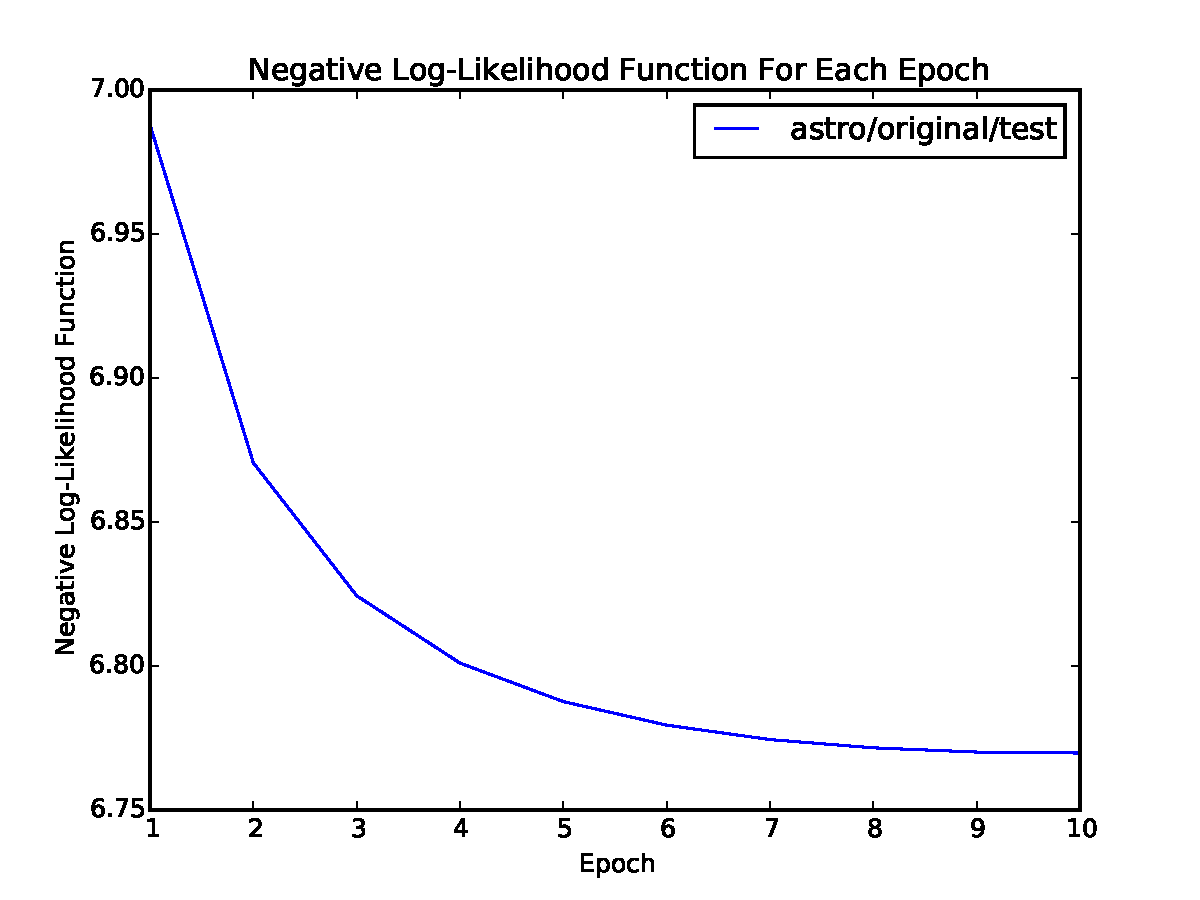
\includegraphics[width=.5\textwidth]{SGD-results-orig2.pdf}
\label{fig:neg_loger_orig}
\caption{Negative Log Likelihood Function of $J(\mathbf{w})$ for original data}
\end{figure}

\begin{figure}[!h]
\centering
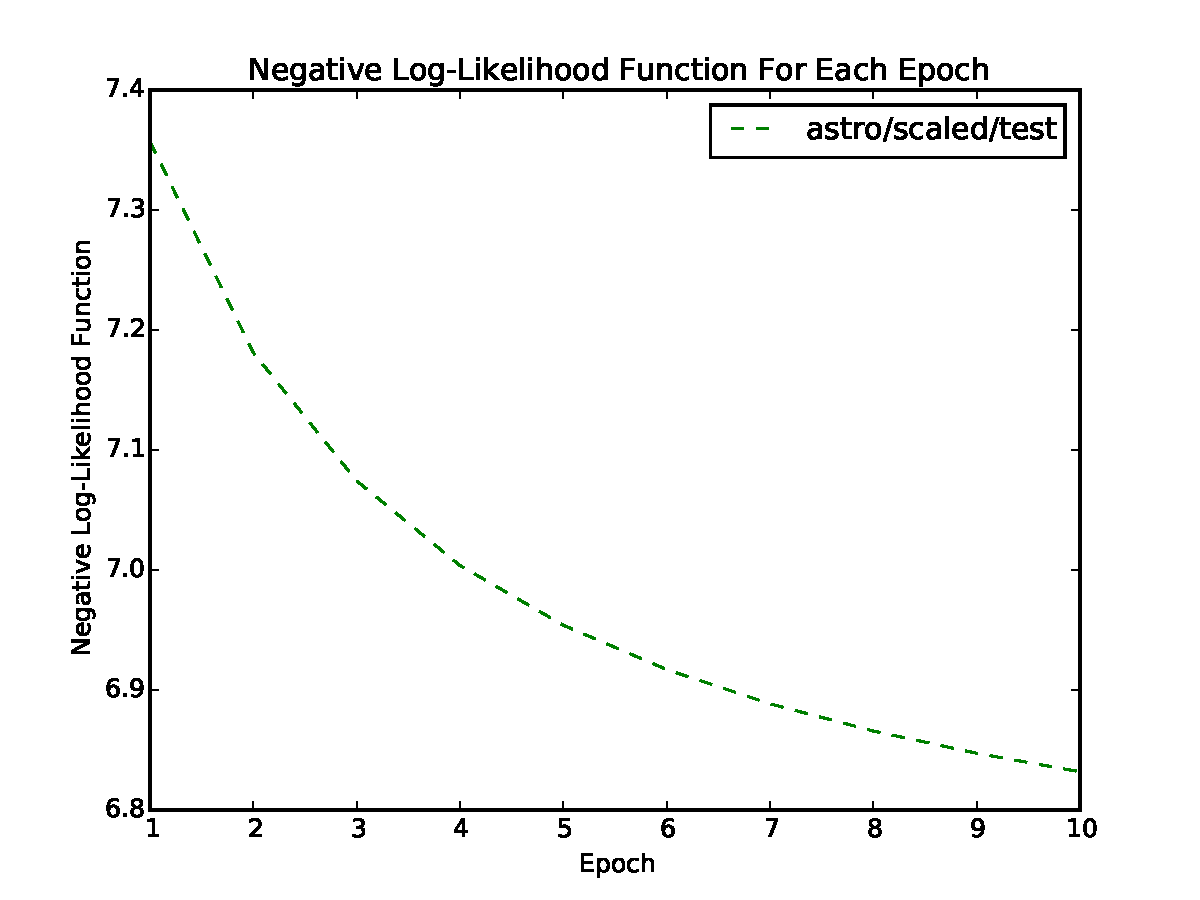
\includegraphics[width=.5\textwidth]{SGD-results-scaled2.pdf}
\label{fig:neg_loger_scaled}
\caption{Negative Log Likelihood Function of $J(\mathbf{w})$ for scaled data}
\end{figure}
\end{enumerate}

{\large \bf Logistic Regression -- Extra Credit}

\begin{enumerate}
\item The gradient of any function is defined as
\begin{align}
\Grad{f(\mathbf{x})} &= \sum_{i=1}^{\mathcal{D}}\frac{\partial f(\mathbf{x})}{\partial x_{i}}\hat{e}_{i}\\
\intertext{where $\mathcal{D}$ is the dimensionality/number of dependent variables in $f(\mathbf{x})$ and $\hat{e}_{i}$ is the normal vector for that coordinate -- a value of 1 for all dimensions in cartesian space. This requires a derivative over $\mathbf{x}$ and $\mathbf{w}$ which is}
\Grad{f(\mathbf{x}_{i})} &= \sum_{i=1}^{\mathcal{D}}\frac{\partial f(\mathbf{x}_{i})}{\partial \mathbf{w}} + \frac{\partial f(\mathbf{x}_{i})}{\partial \mathbf{x}_{i}}\\
\intertext{We can rewrite our equation $f(\mathbf{x}_{i})$ to make it easier to differentiate}
f(\mathbf{x}_{i}) &= \sum_{i=1}^{n}\log\P{1+\exp(-y_{i}\mathbf{w}^{T}\mathbf{x}_{i})} + \frac{\left|\left| \mathbf{w}\right|\right|^{2}}{\sigma^{2}}\\
\intertext{where the derivative of a sum of a function is the sum of the derivative of that function, so the differentials can be brought inside the sum and the respected differentials can be taken and the partial derivative outside the braces denotes that segment representing that differential of $f(\mathbf{x}_{i})$}
\Grad{f(\mathbf{x}_{i})} &= \left\{ \sum_{i=1}^{n}\frac{-y_{i}\mathbf{x}_{i}}{\exp(y_{i}\mathbf{w}^{T}\mathbf{x}_{i})+1} + \frac{2\left|\left|\mathbf{w}\right|\right|}{\sigma^{2}}\right\}_{\frac{\partial f}{\partial \mathbf{w}}} + \left\{ \sum_{i=1}^{n}\frac{-y_{i}\mathbf{w}^{T}}{\exp(y_{i}\mathbf{w}^{T}\mathbf{x}_{i})+1} \right\}_{\frac{\partial f}{\partial \mathbf{x}_{i}}}
\end{align}

\item The Hessian Matrix is defined as
\begin{align}
\boldsymbol{\mathcal{H}}\left(f(\mathbf{x}_{i})\right) &= \left[ \begin{array}{l l}
\frac{\partial^{2}f}{\partial \mathbf{x}_{i}^{2}} & \frac{\partial^{2}f}{\partial \mathbf{x}_{i}\partial \mathbf{w}}\\
\frac{\partial^{2}f}{\partial \mathbf{w} \partial \mathbf{x}_{i}} & \frac{\partial^{2}f}{\partial \mathbf{w}^{2}}
\end{array} \right]\\
\frac{\partial^{2}f(\mathbf{x}_{i})}{\partial \mathbf{x}_{i}^{2}} &= \sum_{i=1}^{n} \frac{\left|\left|\mathbf{w}\right|\right|^{2}y_{i}^{2}e^{\varsigma_{i}}}{\left(e^{\varsigma_{i}}+1\right)^{2}}\\
\frac{\partial^{2}f(\mathbf{x}_{i})}{\partial \mathbf{x}_{i}\partial \mathbf{w}} &= \sum_{i=1}^{n}\frac{y_{i}\left[e^{\varsigma_{i}}\left(\varsigma_{i}-1\right)-1\right]}{\left(e^{\varsigma_{i}}+1\right)^{2}}\\
\frac{\partial^{2}f(\mathbf{x}_{i})}{\partial \mathbf{w} \partial \mathbf{x}_{i}} &= \frac{\partial^{2}f(\mathbf{x}_{i})}{\partial \mathbf{x}_{i}\partial \mathbf{w}} = \sum_{i=1}^{n}\frac{y_{i}\left[e^{\varsigma_{i}}\left(\varsigma_{i}-1\right)-1\right]}{\left(e^{\varsigma_{i}}+1\right)^{2}}\\
\frac{\partial^{2}f(\mathbf{x}_{i})}{\partial \mathbf{w}^{2}} &= \sum_{i=1}^{n}\frac{\left|\left|\mathbf{x}_{i}\right|\right|^{2}y_{i}^{2}e^{\varsigma_{i}}}{\left(e^{\varsigma_{i}}+1\right)^{2}}+\frac{2}{\sigma^{2}}
\end{align}
where $\varsigma_{i} = \mathbf{w}^{T}\mathbf{x}_{i}y_{i}$

\item A matrix is {\em positive semidefinite} if and only if $\mathbf{b}^{T}\boldsymbol{\mathcal{H}}\mathbf{b}>\vec{0}\ \forall\ \mathbf{b}\neq\vec{0}$, where $\mathbf{b}$ is a vector. $\boldsymbol{\mathcal{H}}(f(\mathbf{x}_{i}))$ can be re-written as, by using Einstein Summation Notation
\begin{align}
\boldsymbol{\mathcal{H}} &= \left[ \begin{array}{l l}
\frac{\left|\left|\mathbf{w}\right|\right|^{2}y_{i}^{2}e^{\varsigma_{i}}}{\left(e^{\varsigma_{i}}+1\right)^{2}} & \frac{y_{i}\left[e^{\varsigma_{i}}\left(\varsigma_{i}-1\right)-1\right]}{\left(e^{\varsigma_{i}}+1\right)^{2}}\\
\frac{y_{i}\left[e^{\varsigma_{i}}\left(\varsigma_{i}-1\right)-1\right]}{\left(e^{\varsigma_{i}}+1\right)^{2}} & \frac{\left|\left|\mathbf{x}_{i}\right|\right|^{2}y_{i}^{2}e^{\varsigma_{i}}}{\left(e^{\varsigma_{i}}+1\right)^{2}}+\frac{2}{\sigma^{2}}
\end{array} \right]\\
\intertext{where $\varsigma_{i} = \mathbf{w}^{T}\mathbf{x}_{i}y_{i}$. We only care about if it is going to be negative, so without loss of generality we can remove all the norms, squares, and denominators since they are {\em always} positive. We can also generalize our vector $\mathbf{b}$ as $\mathbf{b} = \left(\alpha_{1},\alpha_{2}\right)^{T}$, where $\alpha_{1}$ and $\alpha_{2}$ can be anything}
\boldsymbol{\mathcal{H}}^{\prime} &= \left[ \begin{array}{l l}
e^{\varsigma_{i}} & e^{\varsigma_{i}}(\varsigma_{i}-1)-1\\
e^{\varsigma_{i}}(\varsigma_{i}-1)-1 & e^{\varsigma_{i}}+\frac{2}{\sigma^{2}}
\end{array} \right]\\
\intertext{where $\mathbf{b}^{T}\boldsymbol{\mathcal{H}}^{\prime}\mathbf{b}$ can be generalized with the following result}
\mathbf{b}^{T} \left[\begin{array}{l l} x_{1} & x_{2}\\ x_{3} & x_{4}\end{array}\right]    \mathbf{b} &= x_{1}\alpha_{1}^{2} + x_{4}\alpha_{2}^{2} + \alpha_{1}\alpha_{2}(x_{2}+x_{3})\\
\intertext{when applied to $\boldsymbol{\mathcal{H}}^{\prime}$ results in}
\mathbf{b}^{T}\boldsymbol{\mathcal{H}}^{\prime}\mathbf{b} &= \alpha_{1}^{2}e^{\varsigma_{i}} + \alpha_{2}^{2}\left(e^{\varsigma_{i}}+\frac{2}{\sigma^{2}}\right) + 2\alpha_{1}\alpha_{2}\left(e^{\varsigma_{i}}(\varsigma_{i}-1)-1 \right)\\
\intertext{Where there's two instances that we need to prove. (1) If $\alpha_{1},\alpha_{2}>0$ then $\alpha_{1}\alpha_{2}(x_{2}+x_{3})>0$ and (2) if $\alpha_{1}>0$ and $\alpha_{2}<0$, then $\alpha_{1}^{2}x_{1}+\alpha_{2}^{2}x_{2}>\alpha_{1}\alpha_{2}(x_{2}+x_{3})$.}
\alpha_{1},\alpha_{2}>0 \Rightarrow \alpha_{1}\alpha_{2}(x_{2}+x_{3})>0\\
\alpha_{1}\alpha_{2}(x_{2}+x_{3}) &= 2\alpha_{1}\alpha_{2}\varsigma_{i}e^{\varsigma_{i}}-2e^{\varsigma_{i}}-2>0\\
&\underbrace{\varsigma_{i}e^{\varsigma_{i}}-e^{\varsigma_{i}}-1}_{>\ 0\text{ if }\varsigma_{i}e^{\varsigma_{i}}>e^{\varsigma_{i}}-1};\quad\varsigma_{i}\neq 0\\
&\Rightarrow \varsigma_{i}e^{\varsigma_{i}}>e^{\varsigma_{i}}-1\\
&\Rightarrow \varsigma_{i}>1-e^{-\varsigma_{i}}\qed
\intertext{where $\varsigma_{i}\geq 1\ \forall\ i$. Now for the alternative case where if $\alpha_{1}>0$ and $\alpha_{2}<0$, that $\alpha_{1}^{2}x_{1}+\alpha_{2}^{2}x_{2}>\alpha_{1}\alpha_{2}(x_{2}+x_{3})$}
\alpha_{1}^{2}e^{\varsigma_{i}}+\alpha_{2}^{2}\left(e^{\varsigma_{i}}+\frac{2}{\sigma^{2}}\right) &> \alpha_{1}\alpha_{2}\left[ e^{\varsigma_{i}}(\varsigma_{i}-1)-1 \right]\\
\left[ \alpha_{1}^{2} + \alpha_{2}^{2} + \frac{2}{\sigma^{2}e^{\varsigma_{i}}}\right] &> \left[ \alpha_{1}\alpha_{2}(\varsigma_{i}-1)-e^{-\varsigma_{i}} \right]\\
\intertext{if $\varsigma_{i}\gg 1$}
\underbrace{\alpha_{1}^{2}+\alpha_{2}^{2}}_{>\ 0} &> \underbrace{\alpha_{1}\alpha_{2}}_{<\ 0}\underbrace{\left(\varsigma_{i}-1 \right)}_{>\ 0}\qed
\intertext{for $\varsigma_{i}\geq 0$ (always)}
\underbrace{\alpha_{1}^{2}+\alpha_{2}^{2}}_{>\ 0}+\underbrace{e^{-\varsigma_{i}}}_{\geq\ 1}\underbrace{\left(\frac{2}{\sigma^{2}}+1\right)}_{>\ 0} &> \underbrace{\alpha_{1}\alpha_{2}}_{<\ 0}\underbrace{(\varsigma_{i}-1)}_{>\ 0}\qed
\end{align}

\item Because the Hessian Matrix of the function is positive-semidefinite, the given function is convex. On top of which, since we are maximizing the function, we are required to step with the gradient and stop when the slope is less than some tolerance $(\epsilon)$. The gradient gives the slope/direction of the greatest change and we ``walk'' in teh direction which makes the gradient zero. We are guarenteed that one exists since the Hessian is positive-semidefinite.
\end{enumerate}

\end{document}
